% !TEX root = ../../presentation.tex
% Architektur: Design

% Fuer uns wichtig: Der Simulator soll architekturunabhaengig sein
% Erster Schritt: wie beschreibt man eine ISA im Abstrakten?
% Erste Idee: Irgendwas mit Vererbung
% Aber: Prefer composition over inheritance (Gang of Four)
% Flexibles Design durch modularen Aufbau, wie RISC-V!
% 1 Architektur = viele Extensions, mit einem Basismodul (wie RV32I)
% 1 Extension = Units + Instruktionen + Zusaetzliche Information

\begin{slide}{Abstrakte Beschreibung einer ISA}
  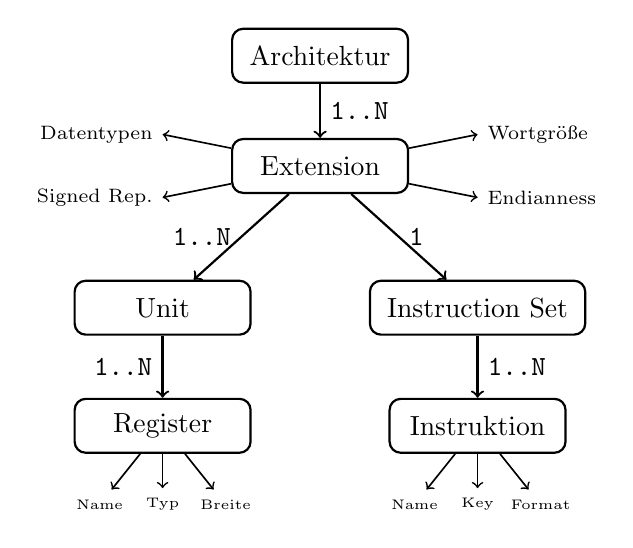
\begin{tikzpicture}[thick]
    \tikzset{block/.style={%
      draw,%
      rectangle,%
      rounded corners,%
      text width=2cm,%
      text height=0.45cm}%
    };
    \tikzset{smallblock/.style={block, text width=1.5cm, text height=0.3cm}};

    %%%%%%%%%%%%%%%
    % Architektur %
    %%%%%%%%%%%%%%%
    \pause
    \path (0, 0.2) coordinate [block] (arch) node {Architektur};

    %%%%%%%%%%%%%%
    % Extensions %
    %%%%%%%%%%%%%%
    \pause
    \path (0, -1.2) coordinate [block] (ext) node {Extension};

    % Edge
    \draw [->] (arch) -- (ext) node [midway, right] {\texttt{1..N}};

    %%%%%%%%%%%%%%%%%%%%%%%%
    % Units (e.g. CPU/FPU) %
    %%%%%%%%%%%%%%%%%%%%%%%%
    \pause
    \path (-2, -3) coordinate [block] (units) node {Unit};
    \draw [->] (ext) -- (units) node [midway, above, left] {\texttt{1..N}};

    % Register
    \pause
    \path (-2, -4.5) coordinate [block] (reg) node {Register};
    \draw [->] (units) -- (reg) node [midway, left] {\texttt{1..N}};


    \pause
    \node (rname) at (-2.8, -5.5) {\tiny Name};
    \node (rtype) at (-2, -5.5) {\tiny Typ};
    \node (rwidth) at (-1.2, -5.5) {\tiny Breite};

    \draw [->, semithick] (reg) -- (rname);
    \draw [->, semithick] (reg) -- (rtype);
    \draw [->, semithick] (reg) -- (rwidth);

    %%%%%%%%%%%%%%%%%%%
    % Instruction Set %
    %%%%%%%%%%%%%%%%%%%
    \pause
    \path (2, -3) coordinate [block, text width=2.5cm]
          (is) node {Instruction Set};

    \draw [->] (ext) -- (is) node [midway, right] {\texttt{1}};

    % Instruktionen
    \pause
    \path (2, -4.5) coordinate [block] (inst) node {Instruktion};
    \draw [->] (is) -- (inst) node [midway, right] {\texttt{1..N}};

    \pause
    \node (iname) at (1.2, -5.5) {\tiny Name};
    \node (ikey) at (2, -5.5) {\tiny Key};
    \node (iformat) at (2.8, -5.5) {\tiny Format};

    \draw [->, semithick] (inst) -- (iname);
    \draw [->, semithick] (inst) -- (ikey);
    \draw [->, semithick] (inst) -- (iformat);

    %%%%%%%%%%%%%%
    % Attributes %
    %%%%%%%%%%%%%%
    \pause
    \draw [->, semithick] (ext) -- (2, -0.8)
          node [right] {\scriptsize Wortgröße};

    \draw [->, semithick] (ext) -- (2, -1.6)
          node [right]{\scriptsize Endianness};

    \draw [->, semithick] (ext) -- (-2, -0.8)
          node [left] {\scriptsize Datentypen};

    \draw [->, semithick] (ext) -- (-2, -1.6)
          node [left] {\scriptsize Signed Rep.}; {\texttt{1}};;
  \end{tikzpicture}
\end{slide}

% Beschreibung der Architektur in YAML Dateien
% Entkoppeln der konkreten *Daten* vom abstrakten Interface
% extends: Schluesselwort erlaubt arbitraere Erweiterung von Extensions
% Ein Graph Algorithmus loest die Abhaengigkeiten einer Architektur zur Runtime
% und bestimmt bzw. merged alle noetigen Extensions

\begin{frame}[fragile]{Definition einer ISA}
  \begin{lstlisting}[style=isa]
                      # RISC-V: RV32I

                      name: rv32i

                      endianness: little
                      word-size: 32
                      signed-representation: twos-complement

                      instructions:
                        - mnemonic: addi
                            length: 32
                            format: I
                            operand length: [0, 0, 12]

                      units:
                        - name: cpu
                          registers:
                            - name: x1
                              id: 1
                              size: 32
  \end{lstlisting}
\end{frame}

\begin{frame}[fragile]{Definition einer ISA}
  \vspace{-0.5cm}
  \begin{lstlisting}[style=isa]
                        # RISC-V: RV64I

                        name: rv64i

                        extends: rv32i
                        word-size: 64

                        instructions:
                          - mnemonic: addiw
                            length: 32
                            format: I
                            operand length: [0, 0, 12]
                            key:
                              opcode: 27
                              funct3: 0
  \end{lstlisting}
\end{frame}
